

\documentclass{article}
\usepackage[utf8]{inputenc}
\usepackage[english]{babel}
\usepackage[]{amsthm} %lets us use \begin{proof}
\usepackage[]{amssymb} %gives us the character \varnothing
\usepackage{graphicx}
\usepackage{hyperref}
\usepackage{multicol}


\title{Homework 4}
\author{Aasim Zahoor}
\date\today


\begin{document}
\maketitle 


\begin{center}
\section{Problems}
\end{center}
\textbf{Link}\vspace{1.5em}
\url{https://github.com/AasimZahoor/Comp_methods.git}
\vspace{1.5em}

\vspace{1.5em}
\textbf{Problem 1}\vspace{1.5em}


This function returns an array where the first element is dP/dr (non relativistic hydrostatic equation)and second one is dM/dr. The variables of the returned functions are P, $M_{enc}$ and r.
    The arguments of this function are:
      \vspace{0.2em}
      
    $k1=G*u_e/l^{3/5}$
    \vspace{0.2em}
    
    $k2=4*pi*u_e/l^{3/5}$
    \vspace{0.2em}
    
        G= Gravitational constant,
        \vspace{0.2em}
        
        c= speed of light,
        \vspace{0.2em}
        
        l= K(the constant multiplied to rho in the relation between P and rho)
        \vspace{0.2em}
        
        $u_{e}=2.$

          \vspace{0.2em}
        \emph{Note: Units given as arguments should be in CGS units.}
  
  \vspace{0.2em}
  
 \textbf{Approach}
 
 We have been asked to solve non relativistic hydrostatic equation for given density range and plot $M_{enc}$ V/s r. I have chosen the density values to be $[10^{4}, 5*10^{4}, 10^{5}, 5*10^{5},10^{6}]$. The max radius is $10^{10}$ cm and the step size is $10^{6} $cm. 
 
 \begin{center}
\begin{multicols}{2}
	\begin{center}
        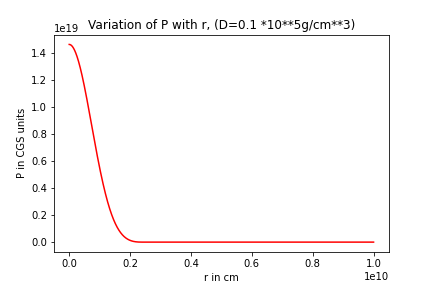
\includegraphics[scale=0.3]{Images/Pr_pb1_0}
        \end{center}
\columnbreak
       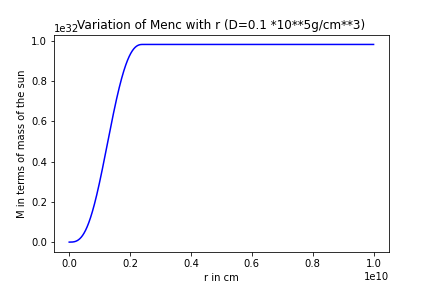
\includegraphics[scale=0.3]{Images/Mr_pb1_0}
\end{multicols}
\begin{multicols}{2}
	\begin{center}
        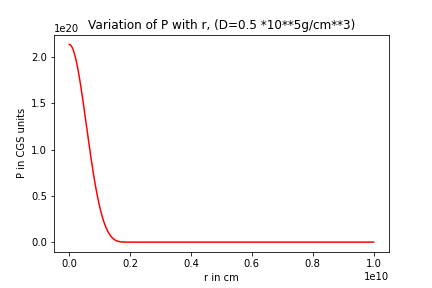
\includegraphics[scale=0.3]{Images/Pr_pb1_1}
        \end{center}
\columnbreak
       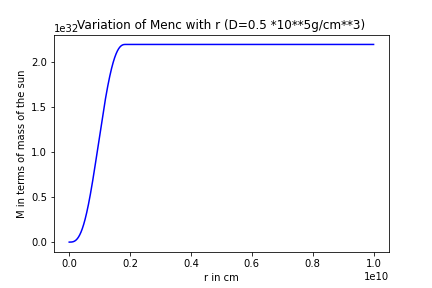
\includegraphics[scale=0.3]{Images/Mr_pb1_1}
\end{multicols}
\begin{multicols}{2}
	\begin{center}
        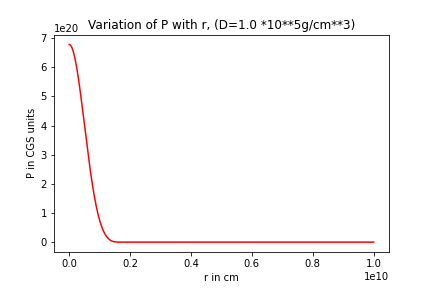
\includegraphics[scale=0.3]{Images/Pr_pb1_2}
        \end{center}
\columnbreak
       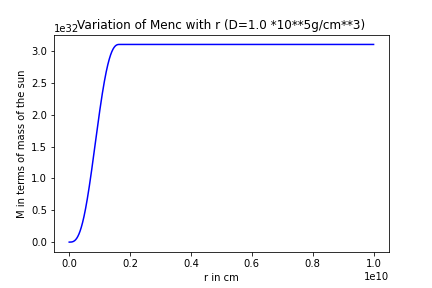
\includegraphics[scale=0.3]{Images/Mr_pb1_2}
\end{multicols}
\begin{multicols}{2}
	\begin{center}
        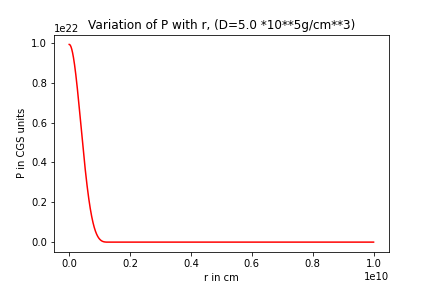
\includegraphics[scale=0.3]{Images/Pr_pb1_3}
        \end{center}
\columnbreak
       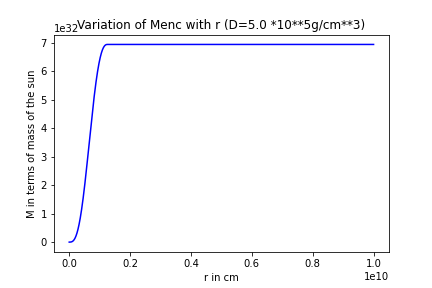
\includegraphics[scale=0.3]{Images/Mr_pb1_3}
\end{multicols}
\begin{multicols}{2}
	\begin{center}
        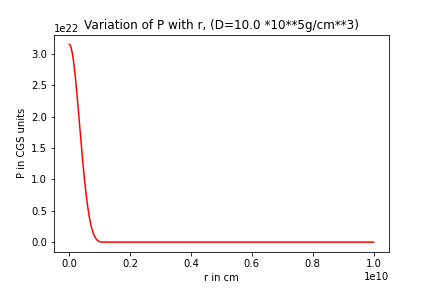
\includegraphics[scale=0.3]{Images/Pr_pb1_4}
        \end{center}
\columnbreak
       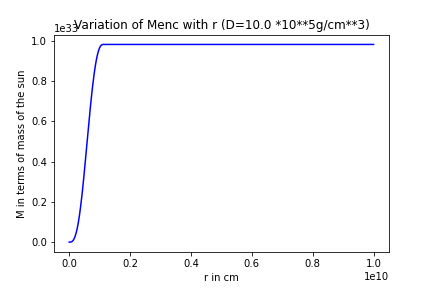
\includegraphics[scale=0.3]{Images/Mr_pb1_4}
\end{multicols}
\textbf{Figure 1}: It is observed maximum mass in reached at lesser radius as density is increased.
\end{center}
\vspace{0.2em}

\clearpage
\vspace{1.5em}
\textbf{Problem 2}\vspace{1.5em}

This function returns an array where the first element is dP/dr (TOV) and second one is dM/dr. The variables of the returned functions are P, $M_{enc}$ and r.
    The arguments of this function are:
      \vspace{0.2em}
      
        G= Gravitational constant,
          \vspace{0.2em}
          
        c= speed of light,
          \vspace{0.2em}
          
        l= K(the constant multiplied to rho in the relation between P and rho).
          \vspace{0.2em}
        \emph{Note: Units given as arguments should be in CGS units.}
  
  \vspace{0.2em}
  
 \textbf{Approach}
 
 We have been asked to solve TOV equation for given density range and plot $M_{enc}$ V/s r. I have chosen the density values to be $[10^{14}, 5*10^{14}, 10^{15}, 5*10^{15},10^{16}]$. The max radius is 20km and the step size is 10 m. 
 
 \begin{center}
\begin{multicols}{2}
	\begin{center}
        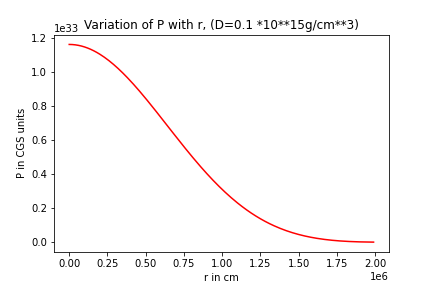
\includegraphics[scale=0.3]{Images/Pr_pb2_0}
        \end{center}
\columnbreak
       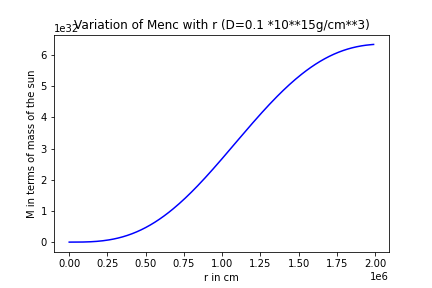
\includegraphics[scale=0.3]{Images/Mr_pb2_0}
\end{multicols}
\begin{multicols}{2}
	\begin{center}
        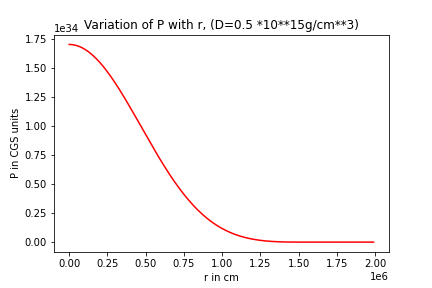
\includegraphics[scale=0.3]{Images/Pr_pb2_1}
        \end{center}
\columnbreak
       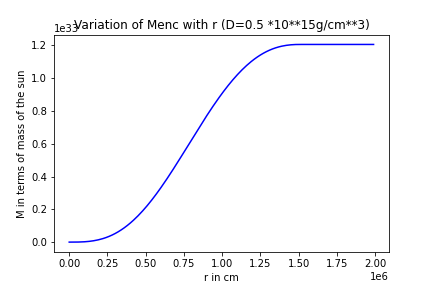
\includegraphics[scale=0.3]{Images/Mr_pb2_1}
\end{multicols}
\begin{multicols}{2}
	\begin{center}
        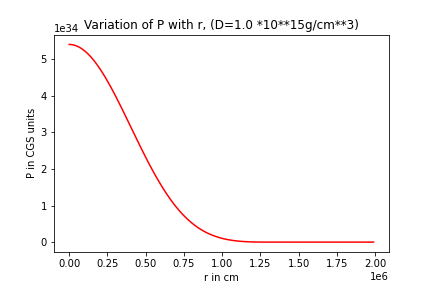
\includegraphics[scale=0.3]{Images/Pr_pb2_2}
        \end{center}
\columnbreak
       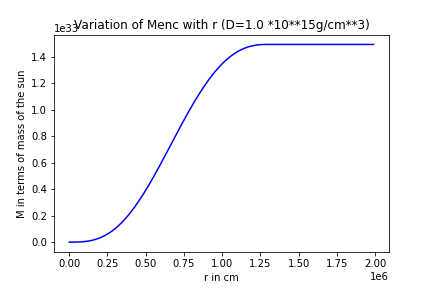
\includegraphics[scale=0.3]{Images/Mr_pb2_2}
\end{multicols}
\begin{multicols}{2}
	\begin{center}
        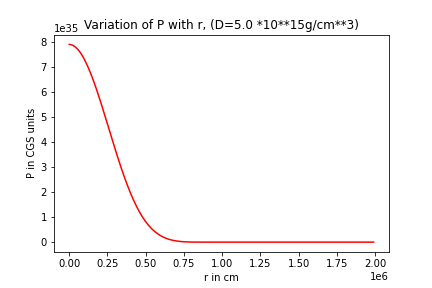
\includegraphics[scale=0.3]{Images/Pr_pb2_3}
        \end{center}
\columnbreak
       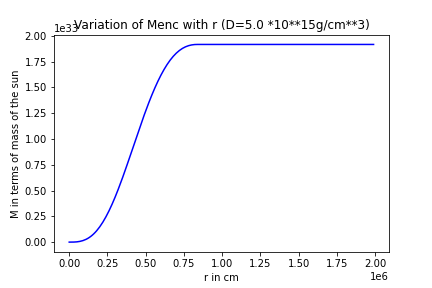
\includegraphics[scale=0.3]{Images/Mr_pb2_3}
\end{multicols}
\begin{multicols}{2}
	\begin{center}
        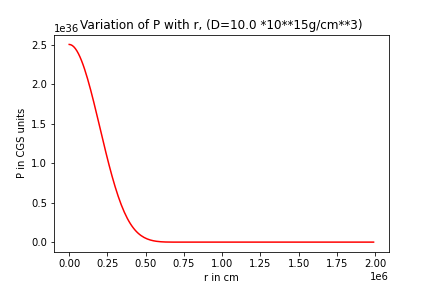
\includegraphics[scale=0.3]{Images/Pr_pb2_4}
        \end{center}
\columnbreak
       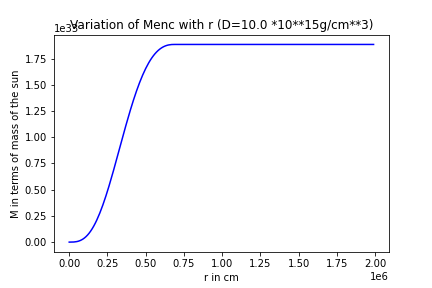
\includegraphics[scale=0.3]{Images/Mr_pb2_4}
\end{multicols}
\textbf{Figure 2}: It is observed maximum mass in reached at lesser radius as density is increased.
\end{center}
\vspace{0.2em}


\textbf{Problem 3}\vspace{1.5em}

In the code for Problem 3 I have defined one function. It is:
  \vspace{0.2em}
  
\begin{itemize}
\item{\textbf{func(G,c,l)}}\vspace{0.2em}

This function returns an array where the first element is dP/dr (TOV) and second one is dM/dr. The variables of the returned functions are P, $M_{enc}$ and r.
    The arguments of this function are:
      \vspace{0.2em}
      
        G= Gravitational constant,
          \vspace{0.2em}
          
        c= speed of light,
          \vspace{0.2em}
          
        l= K(the constant multiplied to rho in the relation between P and rho).
          \vspace{0.2em}
        \emph{Note: Units given as arguments should be in CGS units.}
  
  \vspace{0.2em}
  
 \textbf{Approach}
  
We have been asked to find mass of the Star given radius and using the TOV equation. I approached this problem by assuming density to be $10^(16)g/cm^3$ and then using the TOV equation and $dM_{enc}/dr $ and RK-4 solver to find the values of M and P at different R. Then I found the maximum mass in the returned mass array. I made the code run till $r=13.02 km$ with a step size of 100 cm. Here are the graphs and output:


\emph{\small{}}
\begin{center}
\begin{multicols}{2}
	\begin{center}
        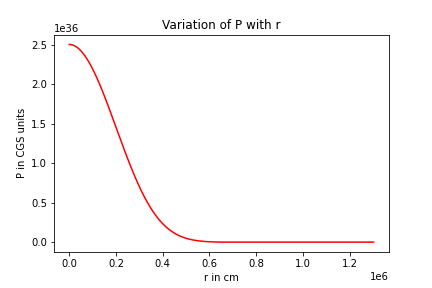
\includegraphics[scale=0.3]{Images/Pr_pb3}
        \end{center}
\columnbreak
       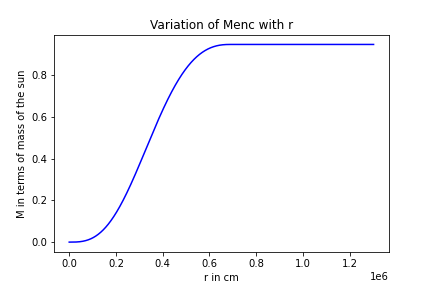
\includegraphics[scale=0.3]{Images/Mr_pb3}
\end{multicols}
\textbf{Figure }: The graphs for problem 3
\end{center}
\vspace{0.2em}
	\begin{center}
        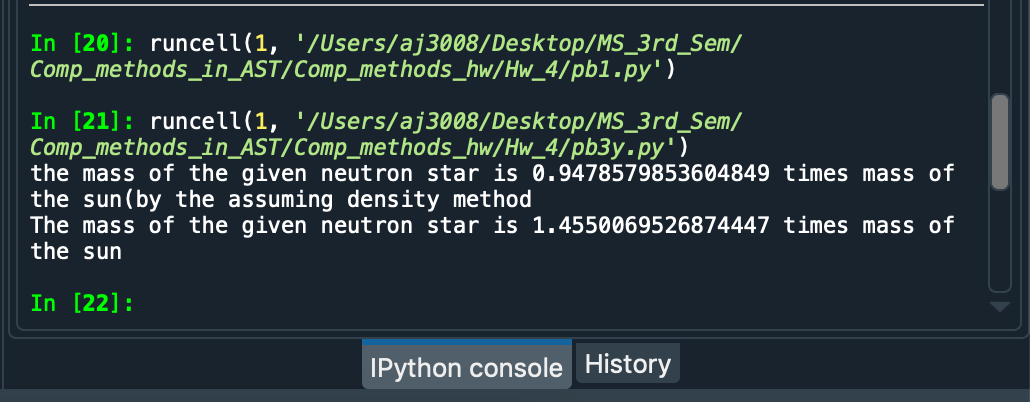
\includegraphics[scale=0.2]{Images/Output_pb3}
          \vspace{0.2em}
          
        \textbf{Figure 3}: The output for problem 3. It is the bottom most value. It reads 0.94785.
        \end{center}
        
     














\end{center}

\vspace{0.2em}
\end{document}
